% Autor: Simon May
% Datum: 2017-10-05
% Diese Datei bietet ein minimalistisches Grundgerüst für ein LaTeX-Dokument,
% z.B. für die Bearbeitung der Aufgaben.
\documentclass[
	% Papierformat
	a4paper,
	% Schriftgröße (beliebige Größen mit „fontsize=Xpt“)
	12pt,
	% Schreibt die Papiergröße korrekt ins Ausgabedokument
	pagesize,
	% Sprache für z.B. Babel
	ngerman
]{scrartcl}

% Achtung: Die Reihenfolge der Pakete kann (leider) wichtig sein!
% Insbesondere sollten (so wie hier) babel, fontenc und inputenc (in dieser
% Reihenfolge) als Erstes und hyperref und cleveref (Reihenfolge auch hier
% beachten) als Letztes geladen werden!

% Silbentrennung etc.; Sprache wird durch Option bei \documentclass festgelegt
\usepackage{babel}
% Verwendung der Zeichentabelle T1 (Sonderzeichen etc.)
\usepackage[T1]{fontenc}
% Legt die Zeichenkodierung der Eingabedatei fest, z.B. UTF-8
\usepackage[utf8]{inputenc}
% Schriftart
\usepackage{lmodern}
% Zusätzliche Sonderzeichen
\usepackage{textcomp}

% Mathepaket (intlimits: Grenzen über/unter Integralzeichen)
\usepackage[intlimits]{amsmath}
% Ermöglicht die Nutzung von \SI{Zahl}{Einheit} u.a.
\usepackage{siunitx}
% Zum flexiblen Einbinden von Grafiken (\includegraphics)
\usepackage{graphicx}
% Abbildungen im Fließtext
\usepackage{wrapfig}
% Abbildungen nebeneinander (subfigure, subtable)
\usepackage{subcaption}
% Funktionen für Anführungszeichen
\usepackage{csquotes}
% Zitieren, Bibliographie
\usepackage{biblatex}


% Verlinkt Textstellen im PDF-Dokument
\usepackage[unicode]{hyperref}
% "Schlaue" Referenzen (nach hyperref laden!)
\usepackage{cleveref}

% siunitx: Deutsche Ausgabe, Messfehler getrennt mit ± ausgeben
\sisetup{
	locale=DE,
	separate-uncertainty
}

 


\begin{document}
\begin{titlepage}
	\centering
	{\scshape\LARGE Versuchsbericht zu \par}
	\vspace{1cm}
	{\scshape\huge Raster-Tunnel-Mikroskopie, Spitzenpräparation und Messungen an Graphit und Gold     \par}
	\vspace{2.5cm}
	{\LARGE Gruppe 6 Mo\par}
	\vspace{0.5cm}
	{\large Nils Kulawiak (E-Mail: n\_kula01@wwu.de) \par}
	{\large Oliver Brune (E-Mail: o\_brun02@wwu.de) \par}
	{\large Anthony Pietz (E-Mail: a\_piet09@wwu.de) \par}
	\vfill
	durchgeführt am 17.12.2018\par
	
	\vfill
	betreut von Alexander Timmer\par
	
	\vfill
	{\large \today\par}
\end{titlepage}

\tableofcontents
\newpage

\section{Kurzfassung}
In diesem Versuch soll ein Stickstofflaser auf verschiedene Eigenschaften untersucht werden. Dazu wird zuerst Energie der einzelnen Impulse, die Repetitionsrate und die Impulsdauer des Lasers bestimmt.


\section{Methode}
Der Stickstofflaser besteht aus zwei gleich geladenen Platten,die über einen Widerstand verbunden sind, und einer Funkenstrecke. Die beiden Platten liegen auf einer leitenden, geerdeten Unterlage, sind jedoch durch eine Folie davon isoliert und funktionieren damit als Elektroden. Zunächst haben die beiden Platten durch Aufladen das gleiche Potential, durch eine Entladung auf die Funkenstrecke entlädt sich eine der beiden Platten schlagartig, was zu einer großen Potentialdifferenz führt. Dadurch kommt es zu einer weiteren Entladung zwischen den beiden Platten an der Stelle, an der sie sich am nächsten sind, wodurch es zu einem Zusammenstoß mit den Stickstoffmolekülen kommt. Deshalb werden die Stickstoffmoleküle angeregt und senden durch hauptsächlich spontane Emission Photonen aus. %bin ich mir nicht ganz sicher nochmal überprüfen pls%

Für die ersten 3 Messungen von Pulsenergie, Repetitionsrate und Impulsdauer des Lasers, sind einfache Messungen mit einer Photodiode, die an einem Oszilloskop angeschlossen ist, nötig.
Bei der Bestimmung der Pulsenergie wird ein einzelner Impuls komplett aufgezeichnet und die niedrigste Spannung herausgesucht, um die Energie zu berechnen. 
Für die Repetitionsrate müssen mehrere Impulse aufgenommen wurden, wodurch über den Abstand der einzelnen Impulse die Rate ausgerechnet wird.
Bei der Impulsdauer wurden wiederum ein Impuls aufgenommen und die Dauer dieses Impulses gemessen.

Die ersten beiden Messungen werden, dabei mit einer "langsameren" Diode gemessen, während für die letztere die schnelle Diode zu benutzten ist. Das ist der Fall, weil die schnellere Photodiode zwar schneller auf Änderungen reagiert, allerdings den Nachteil hat, dass sie ebenso schnell übersteuert.

Der untersuchte Stickstofflaser kommt aufgrund seiner Konstruktionsweise ohne Resonator aus, mit dem normalerweise eine bestimmte Wellenlänge und ein festgelegtes Strahlprofil erzeugt werden. Daher wurde im nächsten Versuchsteil die Divergenz des Strahls bestimmt. Hierzu wurde die Intensität des Strahls an verschiedenen Stellen vertikal entlang des Strahldurchmessers im Abstand von $\SI{30}{cm}$ und $\SI{3}{m}$ zum Laser mit einer Photodiode gemessen. Hierfür wurde im Abstand von $\SI{30}{cm}$ alle $\SI{0,5}{mm}$ ein Messwert genommen, im Abstand von $\SI{3}{m}$ wurde jeden Millimeter ein Messwert genommen. Um Messung in diesem feinen Abständen zu realisieren, wurde die Photodiode auf einem Verschiebetisch positioniert, der senkrecht zum Strahl mithilfe einer Mikrometerschraube verstellt wurde.
Anschließend wurde eine Linse in den Strahlgang gestellt, um den Laserstrahl zu kollimieren. Nun wurde die Messung im Abstand von $\SI{3}{m}$ wiederholt, diesmal wurde alle $\SI{0,5}{mm}$ ein Messwert genommen. Da die Leistung des Laserstrahls stark schwankte, wurde für alle Messungen zur Divergenz am Oszilloskop der Mittelwert der Spannung aus 64 Werten gebildet.

\begin{figure}[h!]
	\centering
	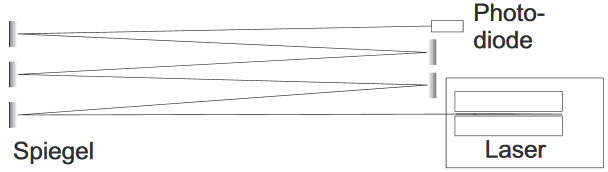
\includegraphics[scale=0.9]{skizze_c.png}
	\caption{Schematische Darstellung des Aufbaus der Messreihe zur Lichtgeschwindigkeit}
	\label{skizze_c}
\end{figure}

Im nächsten Abschnitt sollte mithilfe des Laserstrahls die Lichtgeschwindigkeit bestimmt werden. Dazu wird zuerst der Strahl mithilfe eines Strahlteilers im Abstand von $\SI{13,5}{cm}$ zum Laser teilweise um $90$° abgelenkt. Im um $90$° reflektierten Strahl wurde eine Photodiode im Abstand von $\SI{8,3}{cm}$ platziert. Diese wird mit dem Oszilloskop verbunden. Auch in den nicht reflektierten Strahl wird im Abstand von $\SI{8,3}{cm}$ eine Photodiode platziert. Diese wird auch mit Oszilloskop verbunden, allerdings mit einem deutlich längeren Kabel. Da das Signal im längeren Kabel einen längeren Weg zurücklegen muss als das Signal im kürzeren Kabel, erreichen die Signale das Oszilloskop zu unterschiedlichen Zeiten.
Anschließend wird die zweite Photodiode um drei Meter vom Laser entfernt und die Messung wiederholt. Die Entfernung, die das Licht zur zweiten Photodiode zurücklegen muss, wird nun in Schritten von drei Metern immer weiter erhöht. Hierzu werden, wie in \cref{skizze_c} dargestellt, Spiegel verwendet, die den Laserstrahl über immer größere Strecken zur Photodiode lenken.
Aus der Zeitdifferenz zwischen den beiden Signalen und der Distanz zwischen den optischen Instrumenten lässt sich nun die Lichtgeschwindigkeit bestimmen.

\section{Ergebnis}
Zuerst wird versucht die Pulsenergie des Lasers zu bestimmen. Dazu muss zuerst die niedrigste Spannung ermittelt werden. Um das herauszufinden, wird der niedrigste Weert aus \cref{Energie} genommen. 

\begin{figure}[h!]
	\centering
	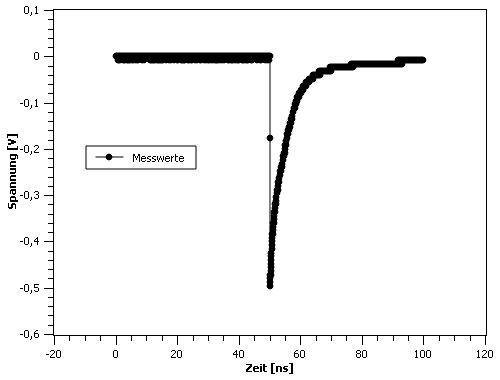
\includegraphics[scale=0.7]{Energie.png}
	\caption{Puls zur Berechnung der Energie}
	\label{Energie}
\end{figure}

Über die Formel
\begin{equation}
E_{p} = \dfrac{1 \mu J}{50mV}U_{min} = \SI{9,92 \pm 0,30}{\mu J} 
\label{eq:Energie}
\end{equation}
lässt sich dann die Energie des Pulses bestimmen.

Die Unsicherheit für die Messung der Spannung liegt bei Einzelmessungen bei 3\%. Daraus folgt die Unsicherheit in \cref{eq:Energie}

Daraufhin soll die Repetitionsrate des Lasers bestimmt werden. Dazu wurden mehrere Pulse in \cref{Rep} aufgenommen und jeweils der Abstand zwischen ihnen bestimmt. Dazu wird jeweils der größte Zeitpunkt gewählt an dem der Puls noch messbar ist und dann die Differenz gebildet. Aus dem Mittelwert ergibt sich eine Repetitionsrate von $t_{Rep}$ = $\SI{0,0814 \pm 0,0006}{s]}$, was einer Frequenz von f = $\SI{12,29 \pm 0,09}{Hz}$ entspricht. Das stimmt auch mit dem vom Oszilloskop abgelesenen Wert von f = $\SI{12,15}{Hz}$ überein.

\begin{figure}[h!]
	\centering
	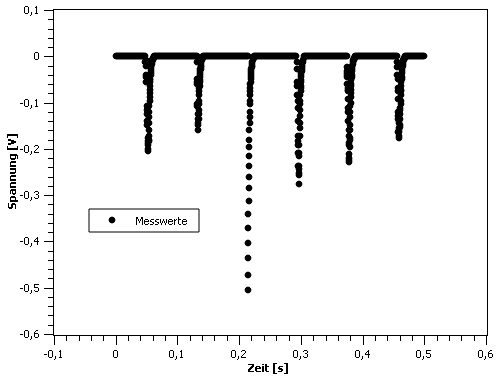
\includegraphics[scale=0.7]{Rep.png}
	\caption{Mehrere Pulse zur Bestimmung der Repetitionsrate}
	\label{Rep}
\end{figure}

Die Unsicherheit von einem Zeitintervall für Einzelmessungen beträgt 
\begin{equation}
u(\Delta t)[\text{s}] = \text{Abtastintervall} + \text{Ablesung} *10^{-4} +0,6*10^{-9}.
\label{eq:ut}
\end{equation}
Aus der Bildung des Mittelwerts folgt die Unsicherheit von $t_{Rep}$.


Als nächstes soll die Impulsdauer eines einzelnen Impulses bestimmt werden. Dies wird mithilfe von \cref{Pulsdauer} versucht. Die Halbwertsdauer lässt sich relativ einfach bestimmen. Dazu wird einfach geschaut, ab wann die Spannung auf die Hälfte des Maximalwertes abfällt. Daraus ergibt sich eine Halbwertsdauer von $t_{\tfrac{1}{2}} = \SI{13,3 \pm 0,6}{ns}$. Schwieriger ist es die Gesamtdauer des Pulses zu bestimmen, da die Spannung für kleine Werte anfängt zu schwanken. Wenn die Gesamtdauer so definiert ist, dass der Puls zu Ende ist, sobald die Spannung unter 0,24V fällt, dann ergibt sich eine Dauer des Gesamtimpulses von $t = \SI{14,180 \pm 0,0014}{ns}$. Die Definition wurde so gewählt, da ab diesem Wert die Spannung anfangen hat stark zu schwanken, allerdings ist diese Definition relativ willkürlich gewählt. 

Die Unsicherheit wurde dabei analog mit \cref{eq:ut} berechnet.

\begin{figure}[h!]
	\centering
	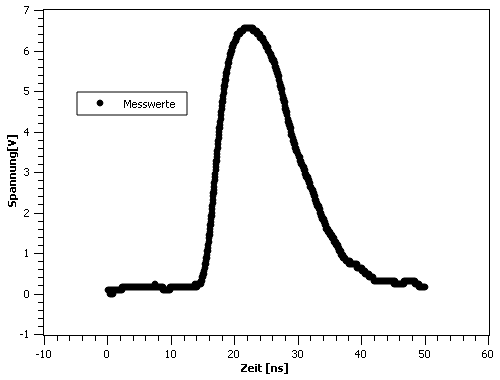
\includegraphics[scale=0.7]{Pulsdauer.png}
	\caption{Genau Auflösung eines Pulses zur Bestimmung der Pulsdauer}
	\label{Pulsdauer}
\end{figure}

\subsection{Divergenz}
Die Intensitätsverteilung des Laserstrahls in unterschiedlichen Abständen vom Laser ist in \cref{breite} dargestellt.

\begin{figure}[h!]
	\centering
	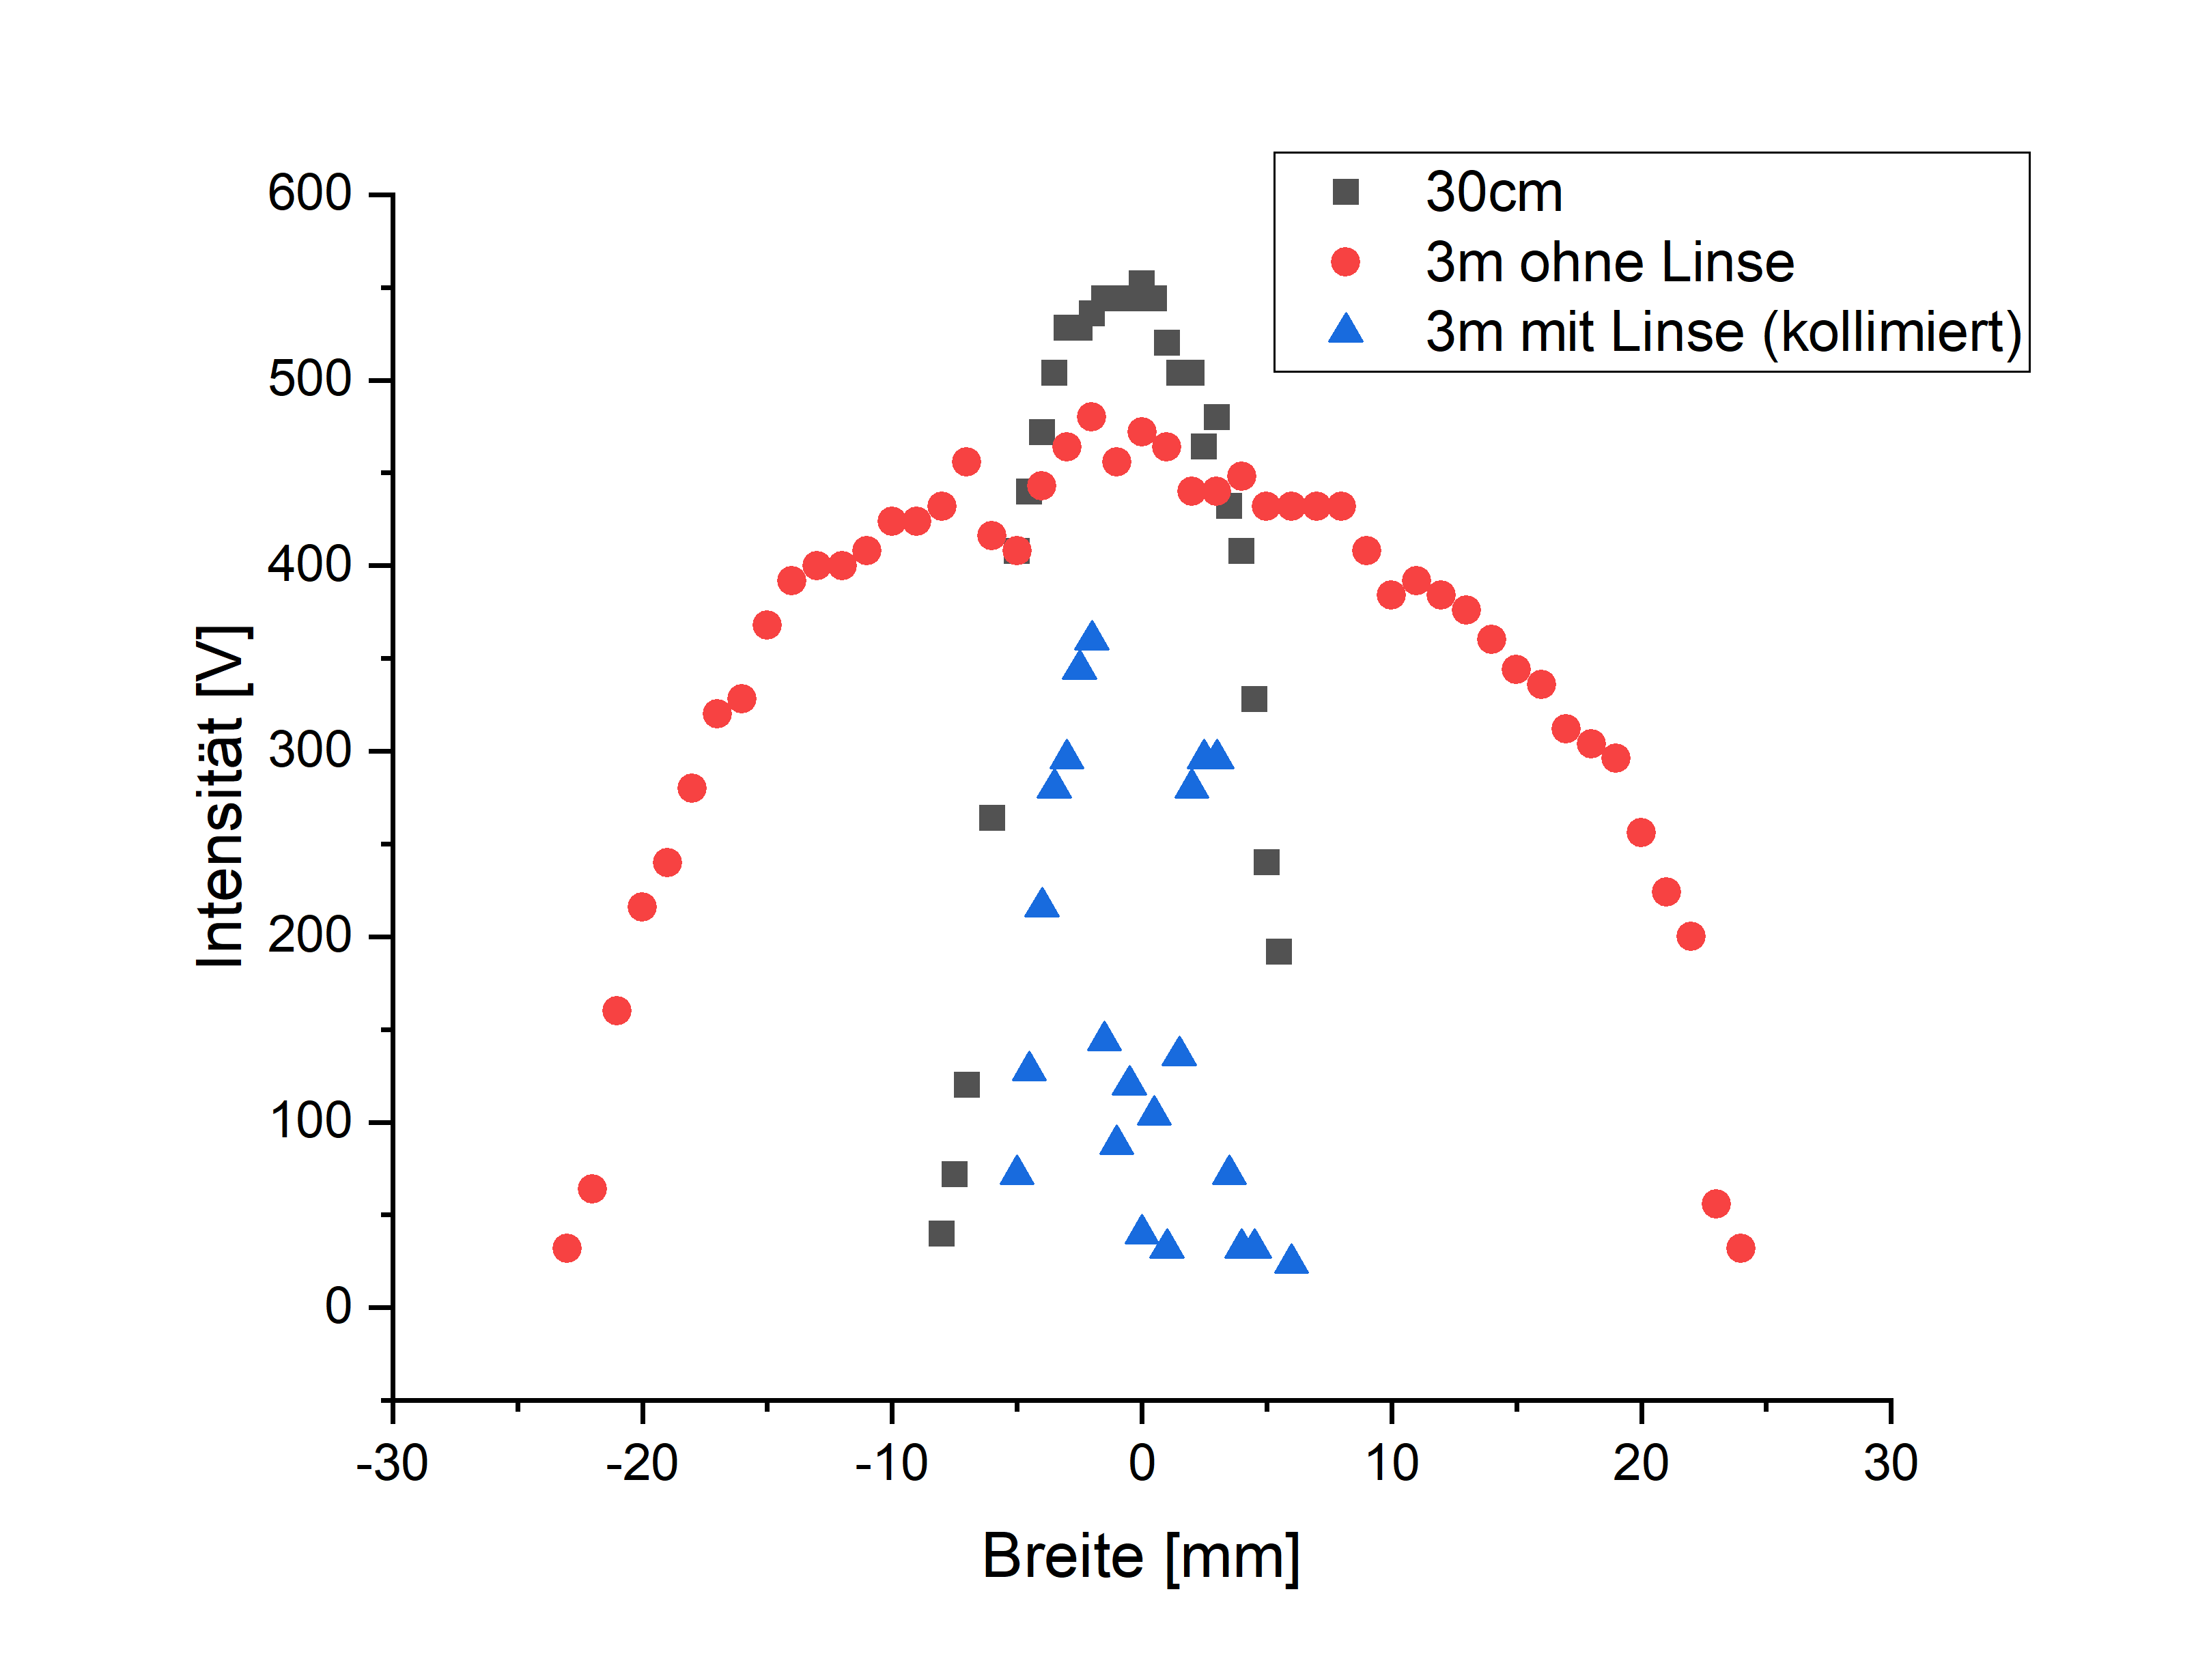
\includegraphics[scale=0.5]{breite.png}
	\caption{Intensität des Laserstrahls aufgetragen gegen den waagerechten Abstand vom Maximum der Intensität in 30cm und 3m Entfernung, einmal mit und einmal ohne Linse im Strahlgang}
	\label{breite}
\end{figure}

Die Messung im Abstand von 30cm ergibt eine schmale, hohe Gaußkurve, da der Laserstrahl an diesem Punkt noch einen kleinen Durchmesser besitzt. In $\SI{3}{m}$ Entfernung ist der Strahl bereits deutlich breiter, außerdem liegt das Intensitätsmaximum etwa $\SI{80}{V}$ niedriger als in $\SI{30}{cm}$ Entfernung. Diese beiden Kurven entsprechen den intuitiven Erwartungen. Die Verbreiterung des Strahls ist auch in \cref{strahlprofil} deutlich sichtbar, wo das Strahlprofil des Lasers linear genähert wurde. Als Rand des Lasers wurden hier die Orte definiert, an denen die Intensität auf die Hälfte des Maximums abgefallen war. Der Strahl verbreitert sich offenbar ohne die Verwendung optischer Instrumente um $\SI{1,056\pm0,025}{mm}$ pro Zentimeter Abstand zum Laser.

\begin{figure}[h!]
	\centering
	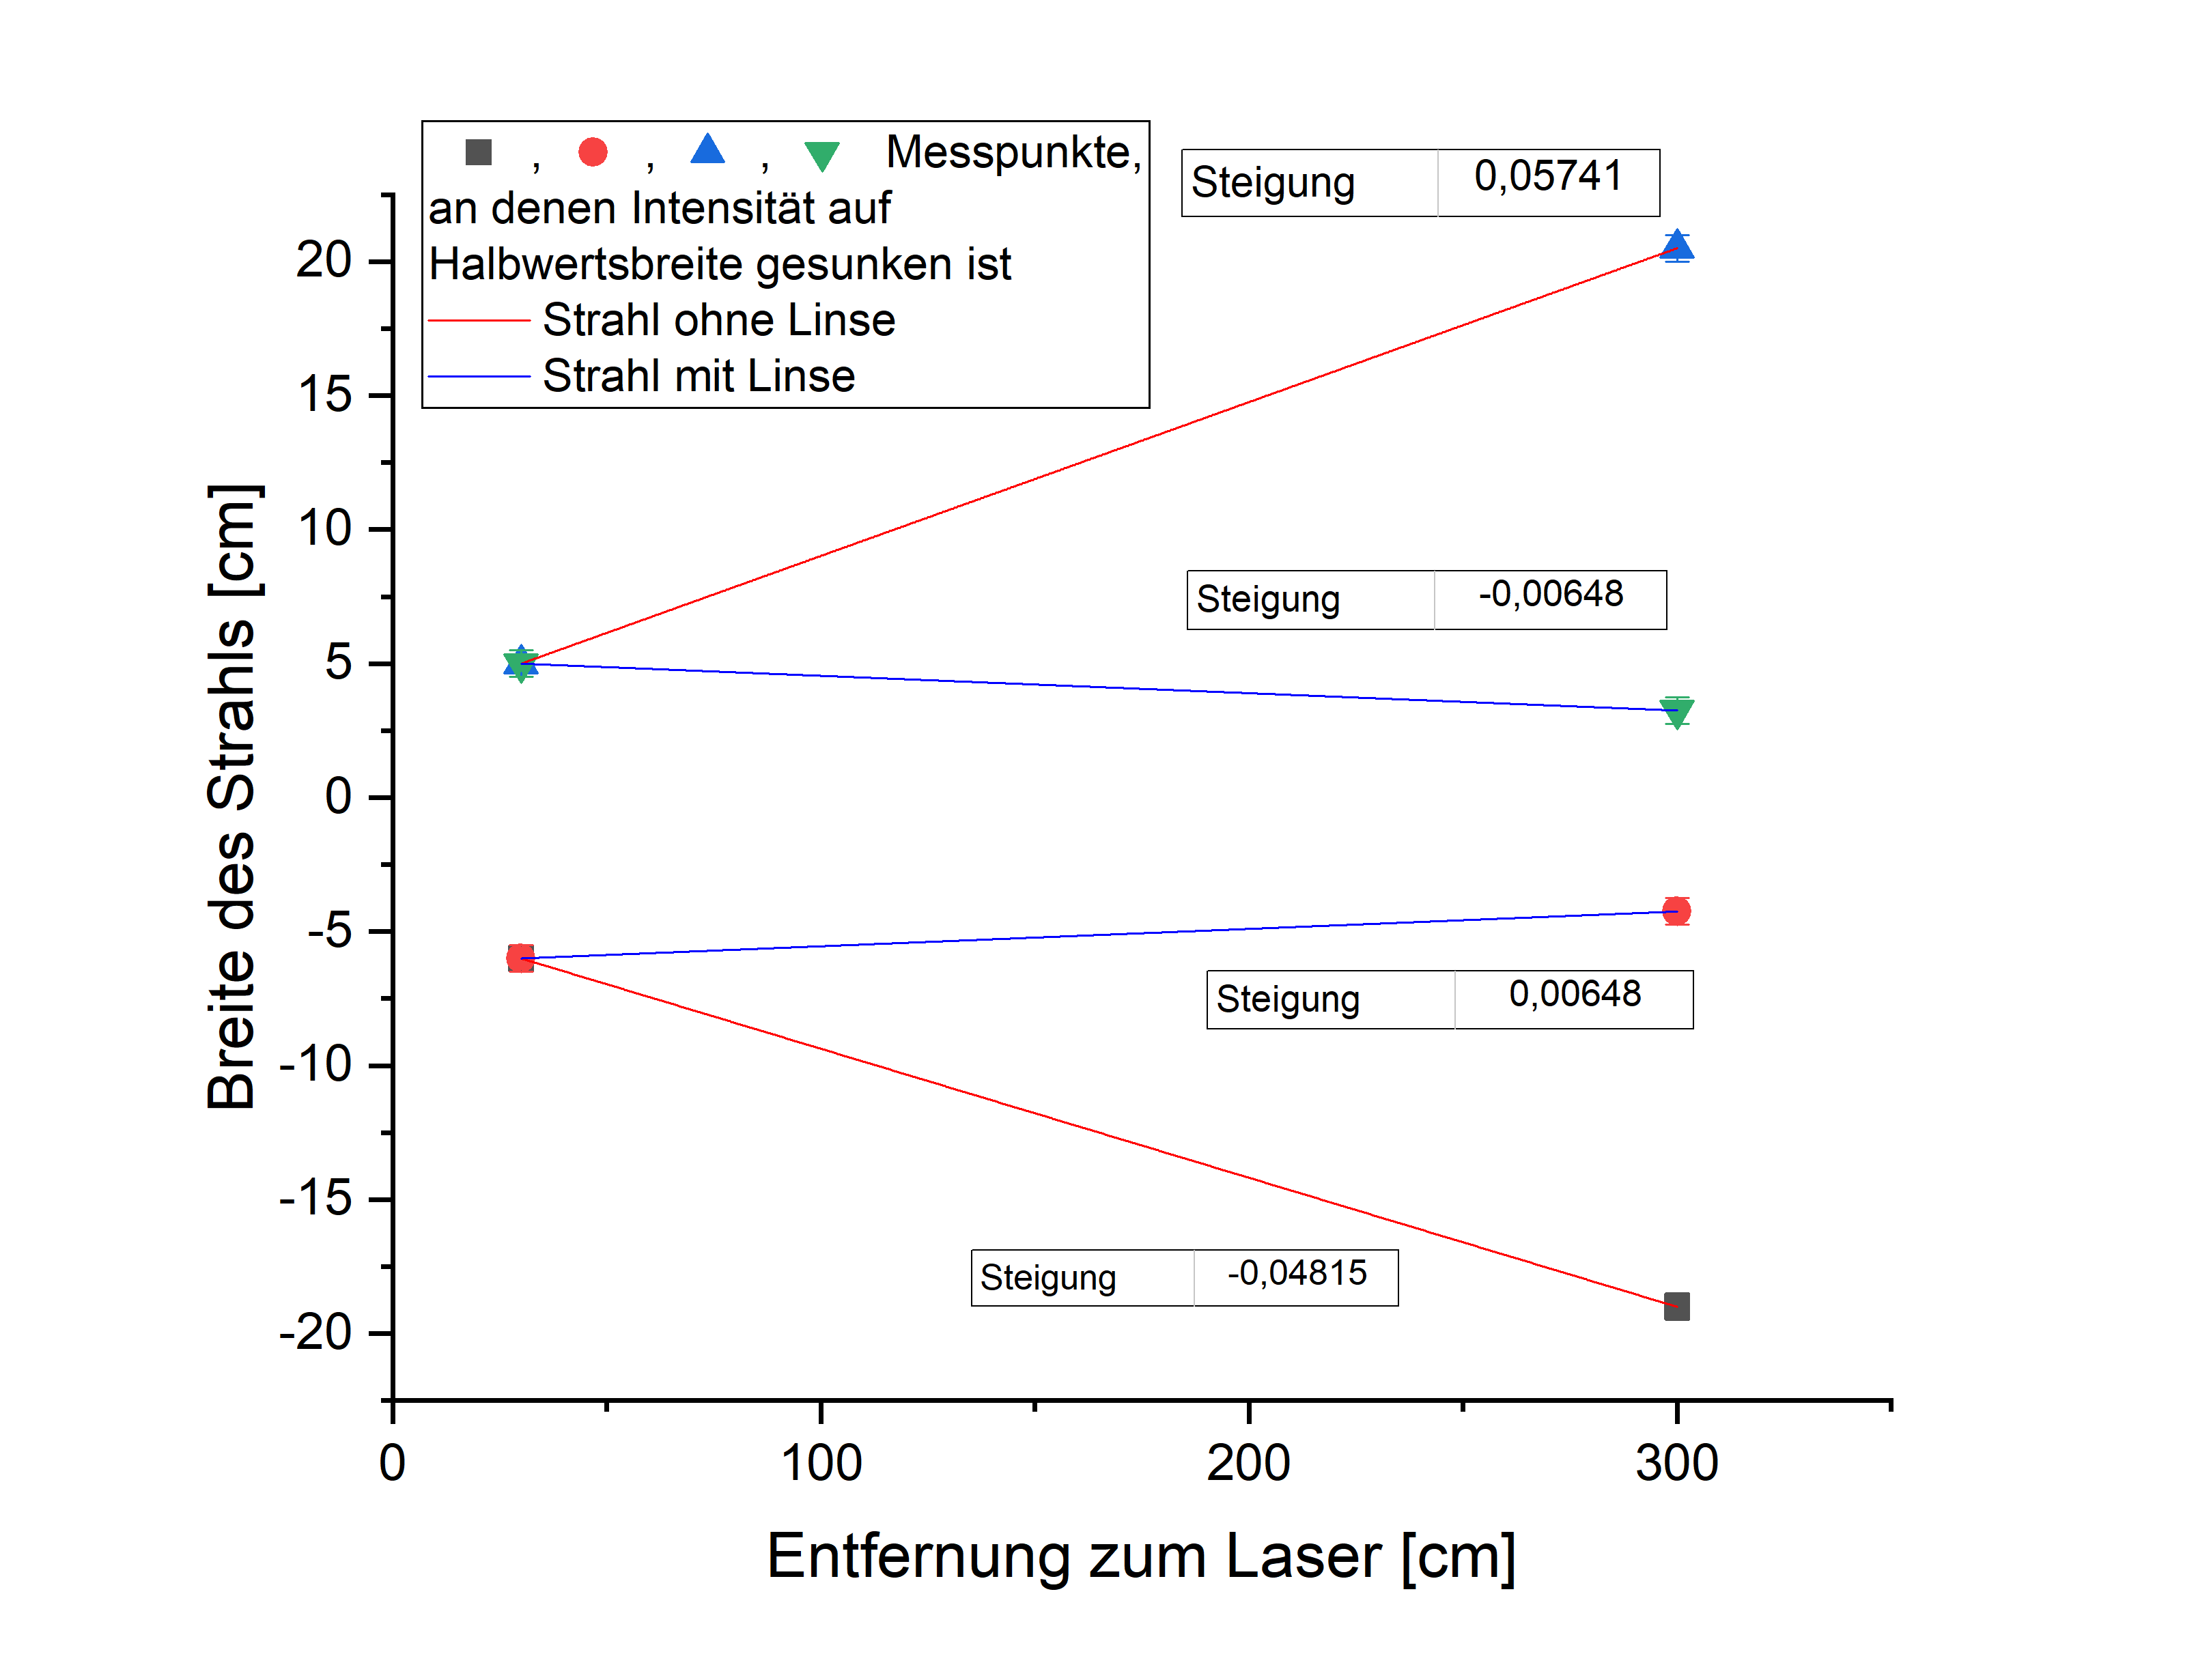
\includegraphics[scale=0.5]{strahlprofil.png}
	\caption{Strahlprofil des unveränderten und des kollimierten Strahls.}
	\label{strahlprofil}
\end{figure}

Um diesen Effekt, der die Strahlqualität deutlich reduziert, zu verhindern, wird nun zur Kollimierung des Strahls in einem Abstand von $\SI{55,5}{cm}$ eine Sammellinse positioniert. Mit dieser Linse im Strahlgang wurde die dritte Messreihe aufgenommen. An den Rändern verhält sich der Laser ähnlich wie in den vorherigen Messreihen, die Intensität steigt zuerst stark an. In der Mitte des Strahls allerdings, wo das Intensitätsmaximum erwartet wird, fällt die Intensität stark ab, sodass der Laserstrahl fast komplett verschwindet. Dieses Verhalten war so nicht erwartet worden, die Intensitätsverteilung weicht stark von der charakteristischen Intensitätsverteilung eines Lasers, wie sie in den beiden vorherigen Messreihen beobachtet werden konnte, ab. Vielmehr ähnelt sie zwei parallel nebeneinander verlaufenden Laserstrahlen.

In \cref{strahlprofil} wurden zur Ermittlung des Strahlprofils die äußeren Halbwertsbreiten zu den beiden Maxima als Breite des gesamten Strahls verwendet. Hieraus ergab sich, dass sich der Strahl hier nicht verbreitert, sondern sogar um $\SI{0,130\pm0,025}{mm}$ pro Zentimeter Abstand vom Laser schmaler wird. Die Linse wurde also nicht optimal positioniert, da sie den Strahl zu stark fokussiert.

Ein möglicher Grund für die untypische Strahlcharakteristik der letzten Messreihe ist, dass die Sammellinse nicht optimal positioniert wurde. Da sie den Strahl nicht nur kollimiert, sondern sogar schmaler werden lässt, wäre es möglich, das die äußeren Anteile des Strahls, die in die Mitte gebrochen werden, mit den Anteilen im Zentrum des Strahls destruktiv interferieren, sodass keine Intensität gemessen wurde. Außerdem lieferte der Laser zu diesem Zeitpunkt des Versuch nur eine sehr stark schwankende Leistung, was die Messwerte weiter verfälscht haben könnte.

Die Unsicherheit bei der Messung der Breite beträgt nur $\SI{\pm0,005}{mm}$, da sich die Position mit der Mikrometerschraube präzise bestimmen ließ, und spielt daher in der Berechnung keine Rolle. Eine etwas größere Rolle spielt die Unsicherheit beim Ablesen der Halbwertsbreite. Da nur alle $\SI{0,5}{mm}$ bzw. alle $\SI{1}{mm}$ ein Messwert genommen wurde, kann die Unsicherheit der Position der Halbwertsbreite auf $\SI{\pm0,5}{mm}$ abgeschätzt werden. Mithilfe der Fehlerfortpflanzung kann so die Unsicherheit der Verbreiterung des Strahls bestimmt werden. Diese beträgt $\SI{\pm0,025}{mm}$.

\end{document}